map计算过程中所产生的中间结果键值对将需要通过网络传送给reduce节点。因此,如果程序产生大量的中间结果键值对,将导致网络数据通信量的大幅增加。而在单词共现算法中,会产生大量的单词对,造成很大的传输开销。为了优化传输开销,我们应该尽量减少传输单词对的数量。为此,在实现细节上,我尝试了三种不同的方案进行比较。
\subsection{baseline}
作为baseline,简单的输出所有单词对,并且单词对是顺序敏感的。即,对于同现的人名A和B,map阶段需同时输出(<A,B>,1)、(<B,A>,1)。
\subsection{WordPair自定义数据类型}
逻辑上来说,单词对应该是顺序不敏感的,<A, B>和<B, A>应该被认为是相同的,在reduce之前应该被划分到同一个节点。这样,单词对的数目就会减少一半。为此,需要自定义一个数据类型WordPair。
\begin{lstlisting}[language=Java]
public class WordPair implements WritableComparable<WordPair> {
	private String word1;
	private String word2;
}
\end{lstlisting}
\indent 由于Hadoop默认使用的Partitioner是HashPartitioner,为了保证相同的主键(不考虑顺序)被发送到相同的reduce节点,我们需要重写自定义类wordpair的hashcode()方法,使得相同的主键的hash值相同。
重写的hashcode方法如下:
\begin{lstlisting}[language=Java]
public int hashCode() {
	return (word1.hashCode()+word2.hashCode())*17;
}
\end{lstlisting}
此外,我们还需重写compareTo()和equals方法使得相同的WordPair键的值可以比较大小和排序。
\subsection{把小的键值对合并成大的键值对}
虽然有Combiner类在每个map节点上合并所产生的中间结果键值对,但观察可发现,在同一个map节点上具有相同主键的键值对并不多,可减少的键值对数量很少。而对于某特定的人名a,与其共同出现的人名有很多,我们可以采用以下的方式将小键值对合并成大的键值对,再在reduce阶段进行累加:
\begin{figure}[htbp]
	\begin{center}
		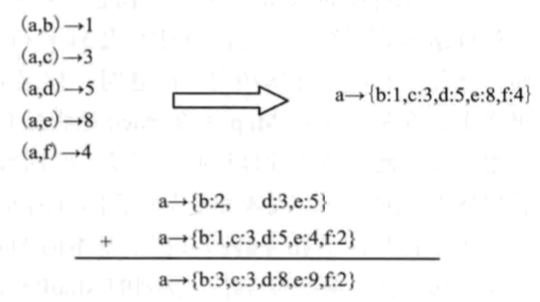
\includegraphics[width=4in]{figures/combine.png}
	\end{center}
\end{figure}
采用这种方法,会减少大量的中间结果键值对。
\subsection{结果对比}
以下表格是分别采用上述三种方法运行单词共现任务的耗时:
\begin{table}[htbp]
	\begin{center}
		\begin{tabular}{|c|c|}
			\hline
			\textbf{方法} & \textbf{单词共现任务耗时} \\ \hline
			baseline    & 66s               \\ \hline
			自定义键值对      & 56s               \\ \hline
			合并键值对       & 45s               \\ \hline
		\end{tabular}
	\end{center}
\end{table}\\
\indent 可看出,我们的优化是确实有效的,另外,采用将小键值对合并成大键值对的优化方法效果要好于自定义数据类型的方法。